\subsectionA{Gith}
Gith are a lanky race of reptilian humanoids that, when erect, stand close to 2 meters tall, but who spend most of their time, bent-over in a crouch that makes them appear to be only 1.5 meter tall. Their lower jaws jut forward and, while toothless, they have sharp, bony ridges that they use to crush and grind their food. Their powerful legs allow them to make great leaps, which they use to move about, walking in an awkward waddle only when they cannot jump or when sneaking up on prey.

\subsubsection{Gith Society}
Gith organize themselves into tribes, with the most powerful member acting as leader. All authority comes from the chief, who has the power of life and death over any member of his tribe. If the chief is killed, the strongest members of the tribe will fight to the death in order to determine who will be the new leader. This trial-by-combat occurs immediately, even if the gith tribe is currently in the middle of a battle with another force.

Most gith tribes inhabit mountainous regions, coming down only to raid the villages of other humanoids or to attack a passing caravan. They are usually interested in entertaining themselves with the suffering of others and with the prospect of a good meal (gith will eat anything organic, preferring meat), but know the value of treasure, especially of psionic and magical items.

Gith speak their own language, which has no alphabet but can be expressed in elvish script.

\begin{figure}[t!]
\centering
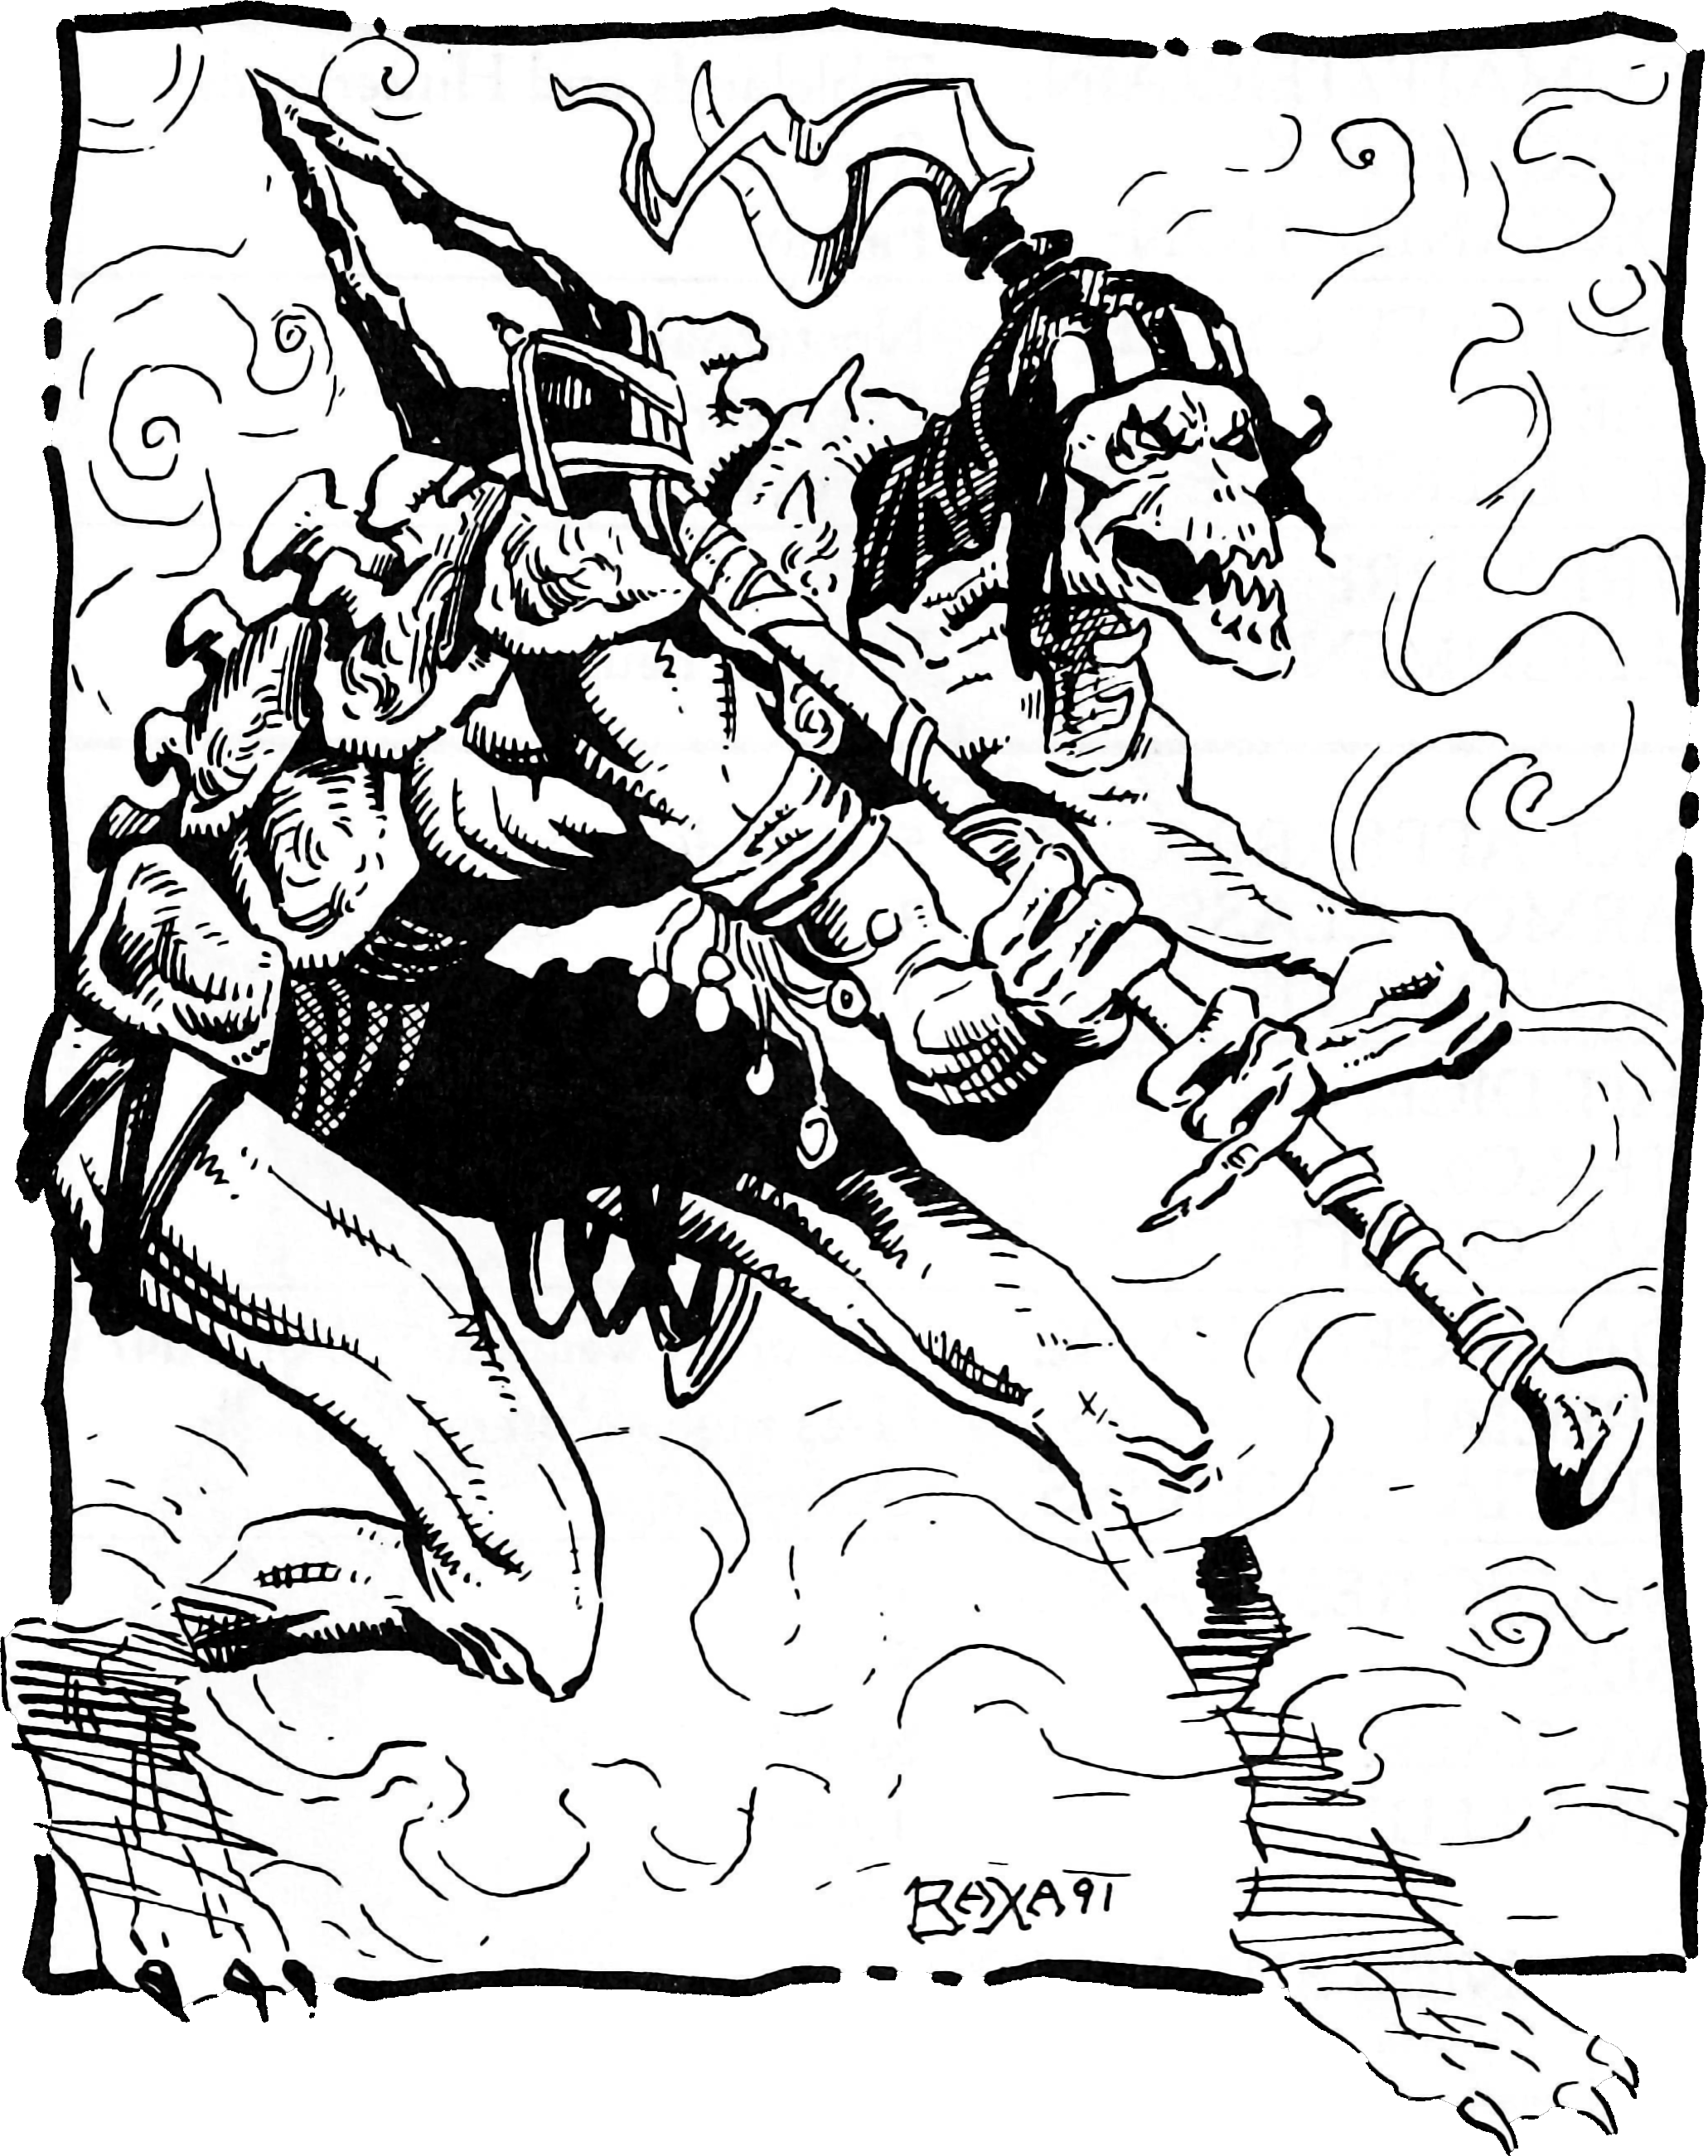
\includegraphics[width=\columnwidth]{images/gith.png}
\WOTC
\end{figure}

\subsubsection{Gith Racial Traits}
\begin{itemize*}
    \item +2 Dexterity, $-2$ Intelligence, $-2$ Charisma: Gith have keen reflexes but are slightly dim and aggressive in their behavior.
    \item Humanoid (gith): Gith are humanoid creatures with the gith subtype.
    \item Medium: As Medium creatures, gith have no special bonuses or penalties due to size.
    \item Gith base land speed is 9 meters.
    \item Low-light vision: Gith can see twice as far as a human in moonlight and similar conditions of poor illumination, retaining the ability to distinguish color and detail.
    \item Natural Armor: Gith have a +2 natural armor bonus to AC due to their tough hide and heavy bones.
    \item Natural Weapons: 2 claws (1d4).
    \item Gith are natural jumpers, gaining a +10 racial bonus to all \skill{Jump} checks.
    \item Leaping Charge (Ex): Gith can use their leap to improve a charge. Whenever a gith charges and they jump at least 3 meters, they gain an additional +2 bonus on their attack roll. This bonus stacks with the +2 bonus given by charging.
    \item Gith have a +4 racial bonus on all \skill{Hide} and \skill{Move Silently} checks. Gith are sly and stealthy.
    \item Automatic Languages: Gith. Bonus Languages: Common, Elven, Pterran, Ssurran and Tarek.
    \item Favored Class: Rogue.
    \item Level Adjustment: +1.
\end{itemize*}
